% $Id$

\section{Implementación}

La siguiente sección presenta los resultados obtenidos
de la implementación de la semántica denotacional
para la extensión probabilística.
De igual manera se describen en esta sección detalles
sobre posibles usos prácticos de la extensión
probabilística.

Han sido utilizados modelos de variabilidad con 1500
características, lo que no permite escribirlos de manera manual.
Para llevar a cabo esta tarea ha sido utilizado el
generador de modelos de características BeTTy~\cite{SeguraHBC11}.
Los parámetros de configuración utilizados en BeTTy han
sido los siguientes: 

\begin{itemize}
        \item La probabilidad de que exista una característica obligatoria es de un 20\%.
        \item La probabilidad de que exista una característica opcional es de un 30\%.
        \item La probabilidad de que una característica este dentro de una relación de \emph{selección única} un 25\%.
        \item La probabilidad de que una característica este dentro de una relación de \emph{paralelo} un 25\%.
\end{itemize}


Existen dos aplicaciones prácticas dentro del
análisis de líneas de productos usando métodos probabilísticos.

La primera es que es posible calcular la probabilidad
de una característica, que permitirá asignar recursos
de manera mas eficiente al probar las
características con mayor probabilidad de ocurrencia
dentro de la línea de productos.

Otra aplicación es la de estimar la cobertura de las
pruebas dentro de las 
líneas de productos ya que es posible
determinar cuantos productos serán abarcados por las 
pruebas, teniendo en cuenta que con este modelo, no 
es posible determinar que porcentaje representan las
características probadas dentro del número total de
características que conforman el producto.

\begin{figure}[h]
        \centering
        \linefigure
        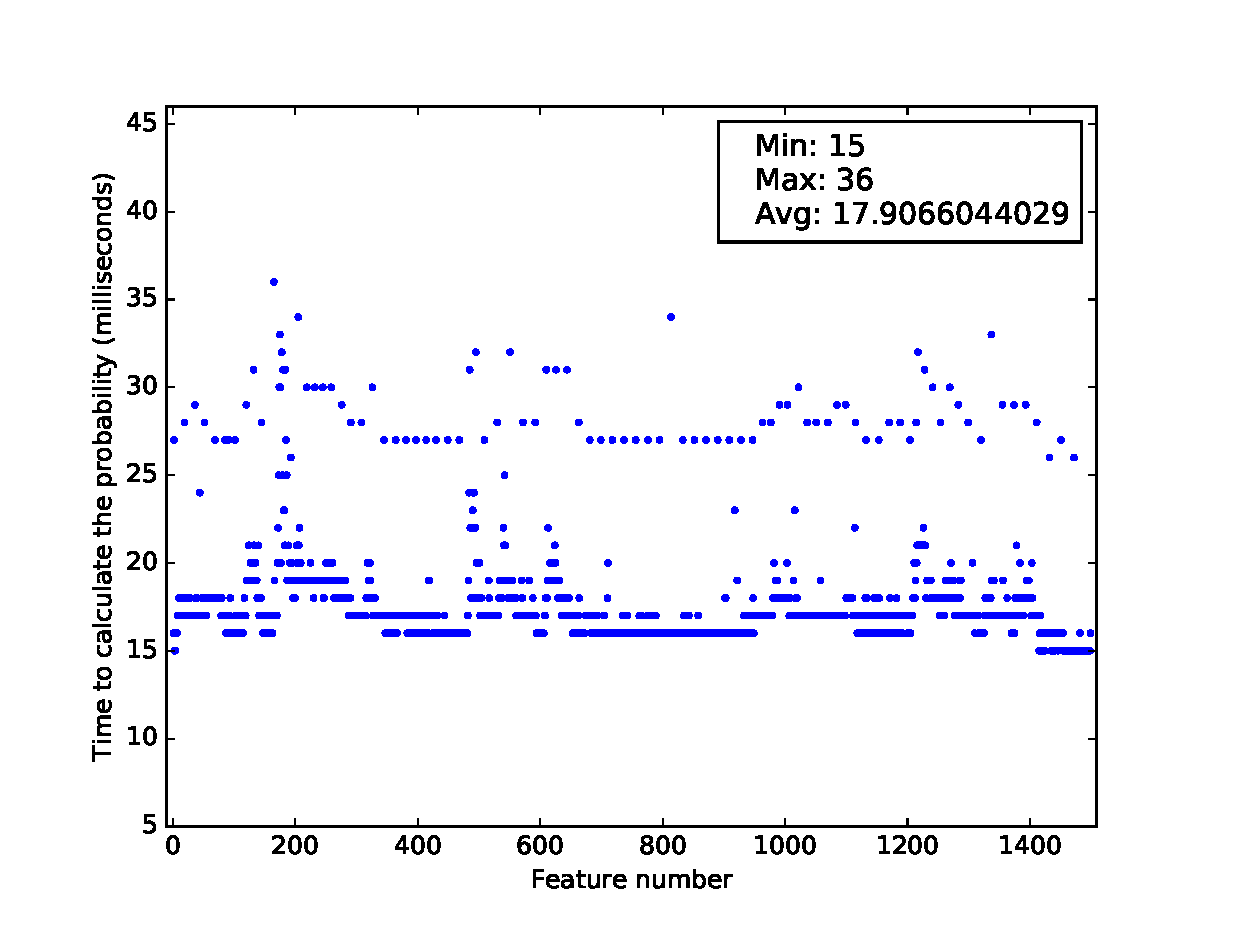
\includegraphics[width=0.8\hsize,angle=0]{chapters/jstat/plot_probs_times.eps}
        \linefigure
        \caption{Tiempo de procesamiento para un modelo con 1500 características}\label{fig:plot:probs:times}
\end{figure}

La figura \ref{fig:plot:probs:times} muestra el tiempo
en calcular la probabilidad de cada característica dentro
del modelo, es importante destacar que los tiempos calculados
son lineales de acuerdo a la longitud del término.
Para todas las características es similar porque para cada
característica debe recorrerse el término completo.

Existe una variación entre el tiempo en calcular la
probabilidad de cada característica y es posible que sea
por el estado actual del nodo donde se ha ejecutado la simulación.

Al ser tiempos de ejecución tan cortos cualquier retraso en 
la planificación del proceso puede tener como consecuencia un
pequeño retraso en su ejecución lo que repercutirá en el resultado
final, esta variación puede considerarse insignificante ya que los
tiempos de ejecución están en el rango de 15 y 38 milisegundos
para cada característica dentro del modelo.

El modelo utilizado en la simulación ha sido ejecutado
en varias ocasiones, teniendo resultados similares en la banda
de 15 y 20 milisegundos, con algunas características procesándose
en la banda superior entre 20 y 38 milisegundos.

\begin{figure}[h]
        \centering
        \linefigure
        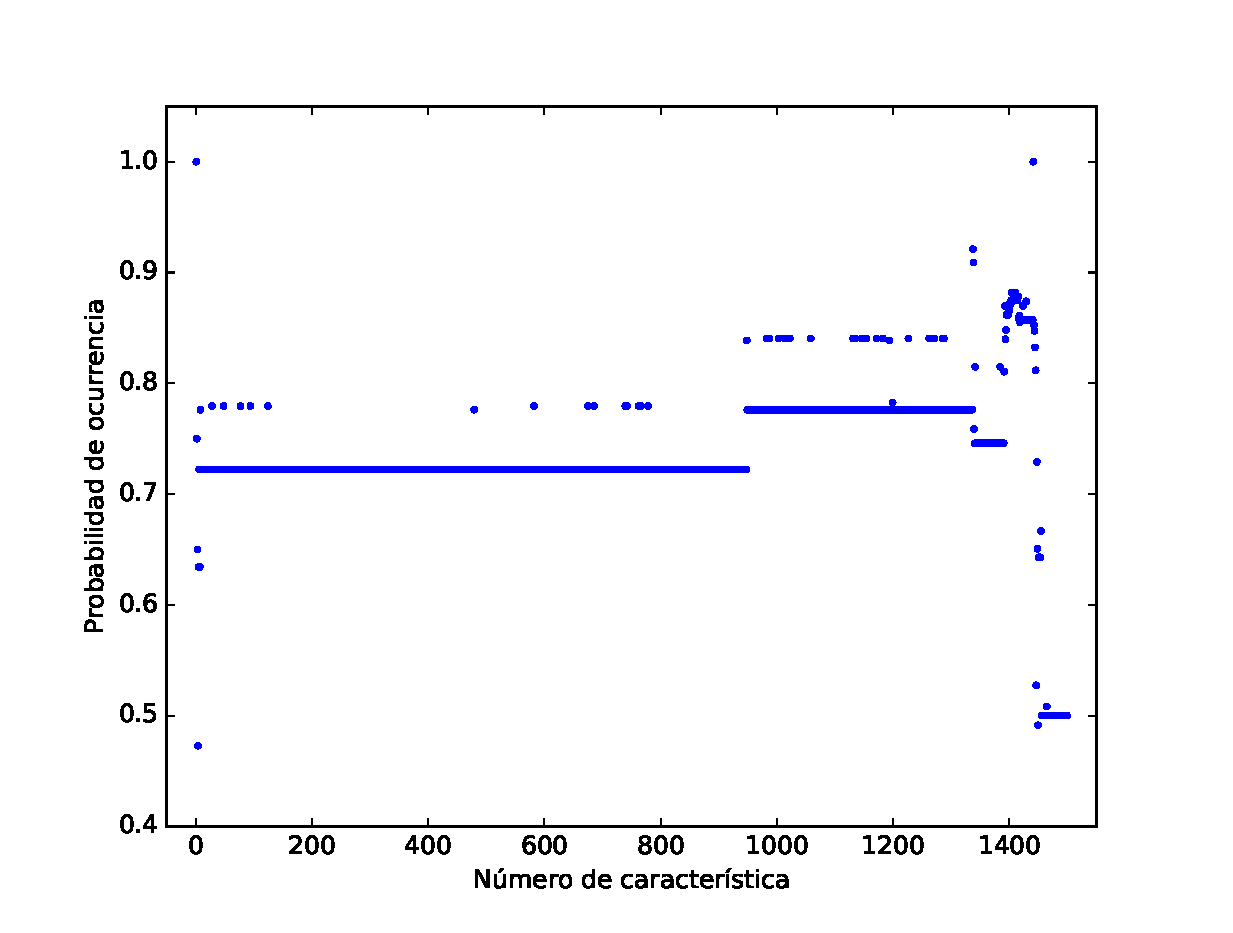
\includegraphics[width=0.8\hsize,angle=0]{chapters/jstat/plot_probs_probs.eps}
        \linefigure
        \caption{Cálculo de las probabilidades para un modelo de variabilidad de 1500 características}\label{fig:plot:probs:probs}
\end{figure}

La figura \ref{fig:plot:probs:probs} muestra gráficamente
la probabilidad de cada característica dentro del modelo
a medida que este se procesa.

Gracias a esta representación gráfica es posible distinguir
claramente agrupaciones de características con mayor probabilidad.


\begin{figure}[h]
        \centering
        \linefigure
        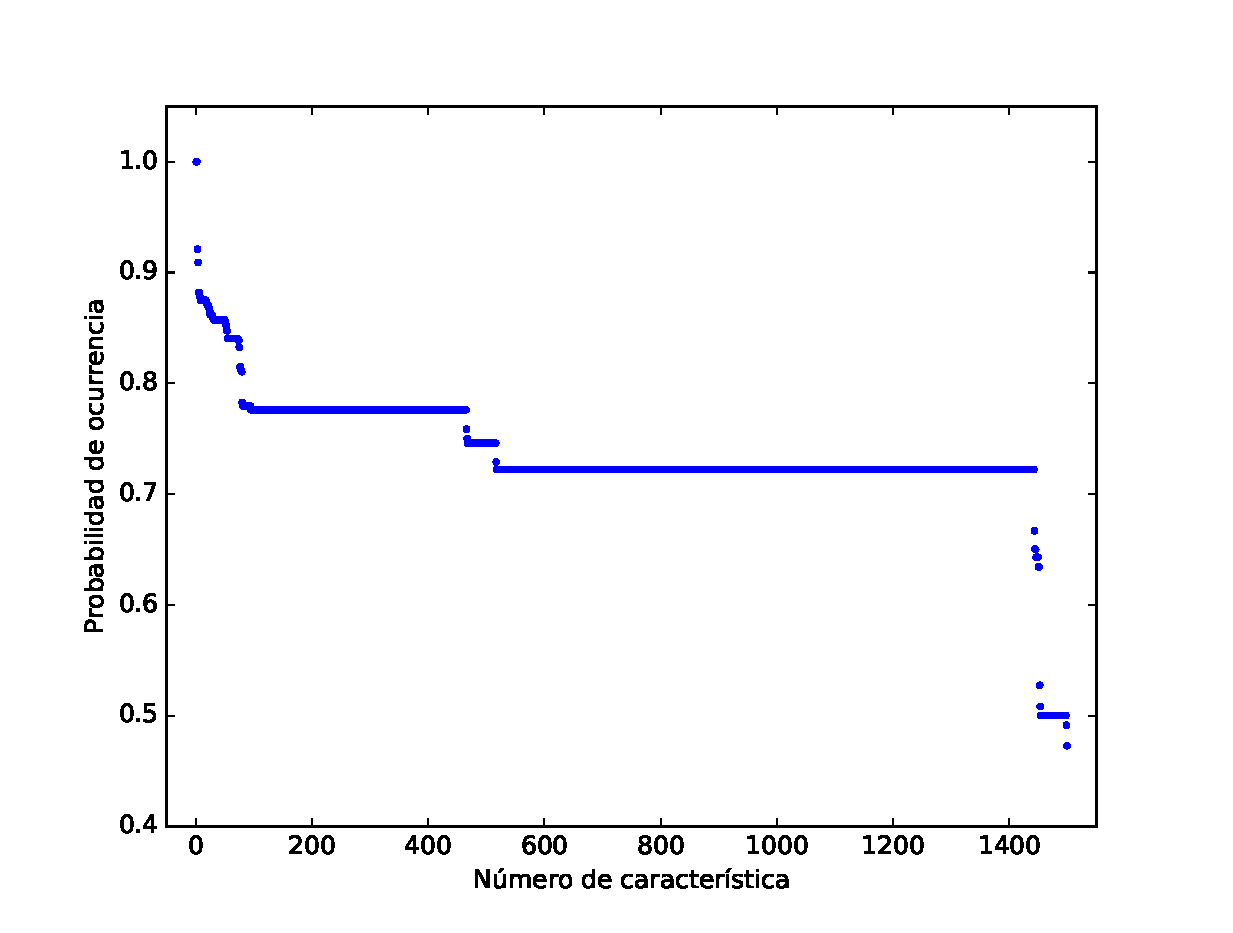
\includegraphics[width=0.8\hsize,angle=0]{chapters/jstat/plot_probs_probs_sorted.eps}
        \linefigure
        \caption{Cálculo de las probabilidades para un modelo de variabilidad de 1500 características ordenadas decrecientement}\label{fig:plot:probs:probs:sorted}
\end{figure}

La figura \ref{fig:plot:probs:probs:sorted} muestra
los resultados de la figura \ref{fig:plot:probs:probs}
ordenados de manera descendiente, esto permite describir con
un detalle mayor aquellas características con mayor 
probabilidad de ocurrencia.

En este caso particular es posible identificar
que aquellas características con probabilidad mayor
a 0.75 se encuentran en solo 450 características
de las 1500 del modelo. Este análisis permitiría
establecer que probando aproximadamente el 28\% de
los componentes de la línea de producto se abarcarían
pruebas sobre componentes que estarían en el 75\%
del total de productos.






 
%\begin{figure}[t]
%$$
%\begin{array}{ccc}
%\mathtt{Test}&\mathtt{Features}& \mathtt{Time}\\
%\#1& \feature{A},\feature{B} & 10\ units\\
%\#2& \feature{C},\feature{D} & 15\ units\\
%\#3& \feature{A},\feature{C},\feature{D} & 8\ units\\
%\#4& \feature{C},\feature{B} & 9\ units\\
%\end{array}
%$$
%\caption{Input parameter: test suite\label{fig:input:parameter}}
%\end{figure}

%We have two open issues:
%\begin{description}
%\item[Unit testing]  Let $P$ be a software product line, and $T_{unit}$ be a 
%  test suite. Each test checks the correctness of a feature (i.e, %\feature{A} or \feature{B}).
%  We can compute the \emph{probability} of a feature. We test before those features with bigger probability.
%  \begin{itemize}
%  \item We can calculate the most frequent set of features in $P$ to test.  
  %\item  We can provide a coverage of the test suite taking into account the percentage of appearance of each feature.
  %\end{itemize}

%\item[Integration testing] We have a test suite $T_{integration}$ where each test checks
%  the integration of a product. 
%  Let us note that the integration of the product $\{\feature{A},\feature{B}\}$  can be different than 
%  the integration of $\{\feature{A}, \feature{B},\feature{C}\}$. 
%  \begin{itemize}
%  \item Which tests of the suite can be applied in this SPL? 
 % \item What is the coverage of each test suite?
 % \end{itemize}


%\end{description}


%Next step is to associate to each integration test the time that 
%it needs to be completed.
%For instance in Figure~\ref{fig:input:parameter} we represent some integration tests and the 
%time that they need to be completed. 



%\begin{quote}
%\emph{Let us consider an integration test suite and a probabilistic SPL $P$.
%If we only have $n$ time units, which is the \emph{best set} of tests 
%to check the correctness of $P$? We say that a test is better than another 
%test if its representativity (the probability to perform these features together) is higher.} 
%\end{quote}

%\bprop
%        The previous problem is NP-hard\ccomen{I propose the transformation into the Subset Sum problem.}.
%\eprop

%Next we define the subset sum problem. 

%\bdfn
%    Let $A = \{a_1, a_2, \ldots, a_n\}$ be a  set of natural numbers and $s$ be  a positive integer. 
%    The subset sum problem checks if there is a subset $A'\subseteq A$ such that:  $$\sum_{a\in A'} = s$$ 
%\edfn

%In our previous problem we have a set of pairs $B=\{(p_{1},t_{1}),(p_{2},t_{2}),\ldots,(p_{n},t_{n})\}$ where
%$p_{i}$ is the probability to perform the test $i$ and $t_{i}$ is the time needed to perform this test, and 
%two constants $P$ and $T$. $P$ will represent a probability value and $T$ a time value.
%We are looking for those pairs $(p_{i},t_{i}),\ldots,(p_{j},t_{j})\in B$ that 
%$$
%\begin{array}{ll}
%p_{i}+\ldots +p_{j} &\geq P\\
%t_{i}+\ldots +t_{j} &\leq T\\
%\end{array}
%$$

%Let us consider that $p_{i}=t_{i}={a_i}$ and $P=T=s$.
%We can rewrite the previous problem into 

%$$
%\left.
%\begin{array}{ll}
%a_{i}+\ldots +a_{j} &\geq s\\
%a_{i}+\ldots +a_{j} &\leq s\\
%\end{array}
%\right\}=
%a_{i}+\ldots +a_{j} = s\
%$$
 
%And we have the subset sum problem\ccomen{Please check because $p_{i}$ and $t_{i}$ can be reals while $s_{i}$ are integers}.


%\begin{enumerate}
%        \item We can create a GA to solve this problem.
%        \item We have that this problem is FPTAS~\cite{Ibarra:1975:FAA:321906.321909}.
%\end{enumerate}



%In order to obtain a set of tests that holds the previous issues, we propose 
%two implementations. 
%The first one is using a dynamic algorithm while the second one to use a genetic algorithm.  

%\subsection{Dynamic algorithm}

% We adapted the dynamic algorithm of 0-1 Knapsack problem 
%to our problem and we implemented it in python.


%We define a matrix $A$, where $A(i,j)$ contains the 
%maximum value that can be attained from considering
%only the sum of the first i tests' probability that need at most j time units. 


%$$
%A(i,j)=
%\left\{
%        \begin{array}{lll}
%        0 &\hspace*{3em}&\si i=0 \lor j = 0\\
%        A(i-1,j) & & \si t_i>j\\
%        \max{(A(i-1,j),p_{i}+A(i-1,j-t_i))} &&\si t_i \leq j
%        \end{array}
%\right.
%$$

%In our case, we will say that $A(n,T)$ is the solution if the sum of the  percentages
%of all elements involved in this solution is bigger than or equal to $P$. Otherwise we do not have a solution.
  

%For instance, in Table~\ref{figure:input:parameters} there are presented a set of 24 
%different tests with their time consuming and its probability.
%For instance the first element, t1,9,150, means the test t1 needs 9 time units to be completed
%and the value associated with this test is 150\footnote{We could put here a measure, the probability or anything}.  

%\begin{table}
%\centering

%\selectfont
%{\tt
%\begin{tabular}{|l|l|l|}
%\hline
%\#1,9,150 & 
%\#2,13,35&
%\#3,153,200\\
%\#4,50,160&
%\#5,15,60&
%\#6,68,45\\
%\#7,27,60&
%\#8,39,40&
%\#9,23,30\\
%\#10,52,10&
%\#11,11,70&
%\#12,32,30\\
%\#13,24,15&
%\#14,48,10&
%\#15,73,40\\
%\#16,42,70&
%\#17,43,75&
%\#18,22,80\\
%\#19,7,20&
%\#20,18,12&
%\#21,4,50\\
%\#22,30,10&
%\#23,90,1&
%\#24,200,150\\
%\hline
%\end{tabular}}
%\caption{Input parameter (test,time,value) for the test selection algorithm.\label{figure:input:parameters}}
%\end{table}

% \begin{figure}[t]
% \centering
% includegraphics[scale=1]{GA_Flowchart_4}
% \caption{Scheme of GA.\label{scheme:genetic:algorithm}}
% \end{figure}





% After executing the dynamic algorithm, with the following input parameters a)
% the data presented in Table~\ref{figure:input:parameters} and T (the maximum time value) equals to 500, 
% we obtain that {\tt \#1, \#2, \#3, \#4, \#5,
% \#7, \#8, \#9, \#11, \#12, \#16, \#17, 
% \#18, \#19} and {\tt \#21}       conforms the final solution, and P =  1130.


% \subsection{Genetic Algorithm}

% Next we perform a genetic algorithm to discover a better solution. 
% The GA structure is in Figure~\ref{scheme:genetic:algorithm}. 
% With this algorithm we obtain values bigger than 1130.






% \subsubsection{Representation}
% We represent the possible solutions (those tests that hold the conditions) as follows:
% \begin{itemize}
%         \item Genotype: Given $n$ tests, we represent a solution with a binary (1/0) string
% of length $n$ where the position i determines whether the ith-test is included or not.
% The genotype space is complete, that is, any valid solution can be mapped in this array.  
%         \item Phenotype: There are only some genotypes that are \emph{correct}. These are
% those that taking the $n'$, with $n'\leq n$ first $1$ bits from left to right of a genotype, we have that the sum of
% the time values associated with these tests is lower than or equal to T, 
% and that the representativity of these tests is $\geq P$.
% \end{itemize}


% \subsubsection{Initial Population}
% We execute the algorithm with the parameters presented in Figure~\ref{fig:parameters:initial:population} in order to show 
% how many initial population do we need.
% There is an interesting effect that this experiment reveals. 
% The first and second graphs indicate that for populations smaller than 50 the chance for premature convergence seems to be rather high. 
% Therefore we will consider that a good candidate for initial population is 500.

% \begin{figure}[t]
% \centering

% \begin{minipage}{0.45\hsize}\centering
%         \textbf{x}=10

% \includegraphics[scale=0.3]{graphs_basea/basea_diff_raw}
% \end{minipage}
% \begin{minipage}{0.4\hsize}\centering

%         \textbf{x}=50
% \includegraphics[scale=0.3]{graphs_baseb/baseb_diff_raw}

% \end{minipage}


% \begin{minipage}{0.45\hsize}\centering
%         \textbf{x}=200

% \includegraphics[scale=0.3]{graphs_based/based_diff_raw}
% \end{minipage}
% \begin{minipage}{0.4\hsize}\centering

%         \textbf{x}=500
% \includegraphics[scale=0.3]{graphs_basec/basec_diff_raw}

% \end{minipage}

% {\centering
% %\fontsize{7}{9}
% %\selectfont

% \begin{tabular}{|l|l|}
% \hline
% Representation  &Binary strings of length n\\
% Recombination   &One point crossover\\
% Recombination probability &     80\\
% Mutation        & Swap Mutator \\
% Mutation probability    & 2\% \\
% Parent selection        & Roulette\\
% Survivor selection      & Generational\\
% Population size         & \textbf{x} \\
% Termination condition   & Terminate the evolution based on the fitness stats\\
% Generations     & 100 \\
% \hline
% \end{tabular}}

% \caption{Comparing initial population\label{fig:parameters:initial:population}.}
% \end{figure}



% \subsubsection{Recombination probability}
% Next we study the effect of changing the recombination probability. 
% In Figure~\ref{fig:parameters:recombination} we show the max fitness, average fitness and 
% minimum fitness of the population, in each generation, using the probability values 0.1, 0.4, 0.8 and 1 for recombination. 
% We will use 0.8 in the rest of experiments because a) we obtain the maximum fitness, and b) the difference between maximum and minimum is low.

% Let us also note that adding more values of recombination probability (i.e, 100\%), that is also presented in 
%  Figure~\ref{fig:parameters:recombination} does not imply to have better fitness solutions. So, this value should be high 
% but not 100\%.

% \begin{figure}[t]

% \centering

% \begin{minipage}{0.5\hsize}\centering
%         \textbf{x}=0.1

% \includegraphics[scale=0.3]{graphs_basee/basee_maxmin_fitness}
% \end{minipage}
% \begin{minipage}{0.4\hsize}\centering

%         \textbf{x}=0.4
% \includegraphics[scale=0.3]{graphs_basef/basef_maxmin_fitness}

% \end{minipage}


% \begin{minipage}{0.50\hsize}\centering
%         \textbf{x}=0.8

% \includegraphics[scale=0.3]{graphs_baseg/baseg_maxmin_fitness}
% \end{minipage}
% \begin{minipage}{0.4\hsize}\centering

%         \textbf{x}=1
% \includegraphics[scale=0.3]{graphs_baseh/baseh_maxmin_fitness}

% \end{minipage}


% {\centering
% %\fontsize{7}{9}
% %\selectfont

% \begin{tabular}{|l|l|}
% \hline
% Representation  &Binary strings of length n\\
% Recombination   &One point crossover\\
% Recombination probability &     \textbf{x}\\
% Mutation        & Swap Mutator \\
% Mutation probability    & 2\% \\
% Parent selection        & Roulette\\
% Survivor selection      & Generational\\
% Population size         & 500 \\
% Termination condition   & Terminate the evolution based on the fitness stats\\
% Generations     & 100 \\
% \hline
% \end{tabular}}

% \caption{Comparing recombination probability\label{fig:parameters:recombination}.}
% \end{figure}

% \subsubsection{Mutation operator}

% We define two mutation operators in the chromosomes. The first one: swap means to change 
% the element i with the element j. The second one: Integer range, means that we change a bit
% randomly.

% In our algorithm we are able to use both mutators operators. 
% In Figure~\ref{fig:parameters:mutation:operator} the effects of executing swap, integer range or both 
% are presented. 

% We can observe that only swap let the fitness score to be regular with respect to the number of generations. 
% When we change randomly a bit in the chromosomes then the fitness score cannot be predictable. 

% \begin{figure}[t]

% \centering

% \begin{minipage}{0.5\hsize}\centering
%         \textbf{x}=Swap

% \includegraphics[scale=0.3]{graphs_basei/basei_maxmin_fitness}
% \end{minipage}
% \begin{minipage}{0.45\hsize}\centering

%         \textbf{x}=Swap and Integer Range

% \includegraphics[scale=0.3]{graphs_basej/basej_maxmin_fitness}

% \end{minipage}

% \begin{minipage}{0.5\hsize}\centering
%         \textbf{x}=Integer Range

% \includegraphics[scale=0.3]{graphs_basek/basek_maxmin_fitness}
% \end{minipage}
% %\begin{minipage}{0.45\hsize}\centering

% {\centering

% %\fontsize{7}{9}
% %\selectfont
% \begin{tabular}{|l|l|}
% \hline
% Representation  &Binary strings of length n\\
% Recombination   &One point crossover\\
% Recombination probability &     0.8\\
% Mutation        & \textbf{x} \\
% Mutation probability    & 2\% \\
% Parent selection        & Roulette\\
% Survivor selection      & Generational\\
% Population size         & 500 \\
% Termination condition   & Terminate the evolution based on the fitness stats\\
% Generations     & 100 \\
% \hline
% \end{tabular}}
% %\end{minipage}

% \caption{Comparing Mutation Operators\label{fig:parameters:mutation:operator}.}
% \end{figure}

% \subsubsection{Parent Selection}

% Finally we compare the parent selection methodology used in our algorithm.
% We implement three kind of selections: Rank, Roulette and Tournament.
% In our experiments we decided to use Roulette because it is always increasing, 
% and it seems that we can continue improving the valuation of the set of tests over time. 
% Moreover the others seem to be saturated. 
% \begin{figure}[t]

% \centering

% \begin{minipage}{0.5\hsize}\centering
%         \textbf{x}=Rank

% \includegraphics[scale=0.3]{graphs_baser/baser_maxmin_fitness}
% \end{minipage}
% \begin{minipage}{0.4\hsize}\centering

%         \textbf{x}=Roulette
% \includegraphics[scale=0.3]{graphs_bases/bases_maxmin_fitness}

% \end{minipage}

% \begin{minipage}{0.50\hsize}\centering
%         \textbf{x}=Tournament

% \includegraphics[scale=0.3]{graphs_baset/baset_maxmin_fitness}
% \end{minipage}

% %\begin{minipage}{0.45\hsize}\centering


% {\centering
% %\fontsize{7}{9}
% %\selectfont
% \begin{tabular}{|l|l|}
% \hline
% Representation  &Binary strings of length n\\
% Recombination   &One point crossover\\
% Recombination probability &     0.8\\
% Mutation        & Swap \\
% Mutation probability    & 2\% \\
% Parent selection        & \textbf{x}\\
% Survivor selection      & Generational\\
% Population size         & 500 \\
% Termination condition   & Terminate the evolution based on the fitness stats\\
% Generations     & 100 \\
% \hline
% \end{tabular}}
% %\end{minipage}

% \caption{Comparing parent selection\label{fig:parameters:parent:selection}.}
% \end{figure}

%%% Local Variables: 
%%% mode: latex
%%% TeX-master: "main"
%%% End: 

